\documentclass[11pt,a4paper]{article}
\usepackage[utf8]{inputenc}
\usepackage[T1]{fontenc}
\usepackage{geometry}
\geometry{left=2.7cm,right=2.7cm,top=2.6cm,bottom=2.6cm}
\usepackage{lmodern,microtype,setspace}
\usepackage{graphicx,float,amsmath,amssymb,cite,listings,xcolor,booktabs,array,caption,subcaption,algorithm,algpseudocode,tikz,pgfplots,seqsplit}
\usepackage[hidelinks]{hyperref}
\pgfplotsset{compat=1.18}
\usetikzlibrary{shapes,arrows,positioning,fit,backgrounds,matrix,calc}
\onehalfspacing
\setlength{\parindent}{1.5em}
\setlength{\parskip}{0.15em}
\hypersetup{
  pdftitle={Privacy Lens: An Evidence-Bounded Android Privacy Review Framework, Revision 15},
  pdfauthor={Zhiheng Zhang}
}
\title{Privacy Lens: An Evidence-Bounded Android Privacy Review Framework with Governed Legal-Evidence Packs (Revision 15)}
\author{Zhiheng Zhang}
\date{August 2026}
\begin{document}
\maketitle
\begin{abstract}
\small\singlespacing
Mobile privacy-review tools face an evidence-to-decision gap: a permission observation can indicate activity, but it cannot by itself establish purpose, necessity, lawful basis, acquisition completeness, or legal compliance. When an interface suppresses these missing facts, a technically correct calculation can still produce an unreliable conclusion. This thesis addresses that gap through Privacy Lens, a local-first Android prototype that converts bounded permission-audit summaries into traceable prompts for human review.

Following a design-science method, the architecture treats provenance, temporal scope, missing context, and uncertainty as first-class evidence rather than treating a count as a legal verdict. A fail-closed engine rejects malformed records and unsafe temporal aggregation, isolates simulator data, and records the rule-pack version applied to each finding. The European Union General Data Protection Regulation provides the evaluated legal objective; jurisdiction-specific mappings remain outside the Android, repository, and interface layers through a replaceable pack contract.

The implemented product organises the review journey around Overview, Findings, and Settings. Findings remain on the device, Android backup and remote updates are disabled, the evaluated predecessor package has no network or sensitive runtime permission, and users can clear local evidence directly. Revision 15 adds source-status records, calendar-valid governance dates, basis-specific Article 6 evidence, transparency, minimisation, retention-justification, and DPIA-screening questions. A withdrawn-consent signal is labelled a potential conflict for urgent human review, not a finding of infringement.

Evaluation separates rule conformance, hostile admission, temporal behaviour, pack identity, legal-evidence completeness, release packaging, manifest facts, physical installation, and rendered interface evidence. In a fixed-seed 1,000-case corpus, the engine produced 800 true positives and 200 true negatives without disagreement against the specified threshold oracle. A further 1,800 independently calculated pack cases, basis-specific and DPIA evidence probes, governance mutations, accessibility contracts, and release-privacy contracts passed. The 1.3.0 ARM64 APK and AAB built successfully; the APK completed five cold-start rounds on one OPPO PERM00 without a package-specific crash-buffer entry.

These results establish an initial store-submission engineering candidate within the recorded scope. They do not establish legal compliance, unrestricted Android visibility, population accuracy, accessibility conformance, long-run reliability, or store approval. The contribution is an evidence-bounded architecture and traceability method that separate statutory motivation, engineering heuristics, observed evidence, missing legal facts, and prohibited conclusions.
\end{abstract}
\newpage
\tableofcontents
\newpage
\input{Iteration-V2/Chapter1/chapter-01-15}
\section{Literature Review and Foundations}

This chapter examines four bodies of work that constrain the design: data-protection principles, Android observation mechanisms, human-centred warning design, and replaceable rule systems. The purpose is not to claim that Privacy Lens supersedes specialised legal, static-analysis, or enforcement tools. It is to identify the unresolved integration problem between a bounded technical observation and the conclusion a user is invited to draw from it.

\subsection{Review Protocol and Source Quality}

The chapter uses a structured scoping review rather than claiming a systematic review or meta-analysis. Sources were selected to answer four design questions: what a permission observation can establish, which legal facts it omits, how people interpret permission and warning interfaces, and how a replaceable decision mechanism can remain auditable. The search was updated through 10 August 2026 and included official EU and Android material, peer-reviewed security and usable-privacy studies, standards, and foundational information-systems research. Seminal older work was retained when it defined a construct still used in the design, such as contextual integrity, cognitive load, trust calibration, usability, or design science.

Source authority was ranked by the proposition being supported. Statutory meaning is grounded in the GDPR text and final EDPB guidance, not vendor summaries. Platform capability is grounded in Android documentation and bounded by installed-device evidence. Behavioural claims use original field or user studies and preserve their sample sizes and contexts. Engineering-method claims use original design-science publications. Standards and NIST privacy-engineering material are used as design guidance, not as proof of legal compliance \cite{nist8062,nistprivacy2020}. Consultation materials are retained only when their non-final status is explicit; they do not displace binding law or final guidance. Commercial forecasts, uncited practitioner claims, and sources whose title or bibliographic record could not be verified were excluded from the Revision 15 argument.

This protocol has limits. It does not report database-by-database recall, duplicate screening, or a PRISMA flow, and therefore must not be read as exhaustive coverage of mobile privacy research. Its purpose is narrower: make each source class and its evidential role explicit so that a reviewer can distinguish legal authority, platform specification, empirical user evidence, and design rationale.

\subsection{Regulatory Principles and Technical Signals}

The GDPR regulates processing rather than permission counts. Article 5 establishes principles including lawfulness, transparency, purpose limitation, data minimisation, accuracy, storage limitation, integrity, confidentiality, and accountability. Articles 6 and 9 concern lawful bases and special-category data; Article 25 requires data protection by design and by default \cite{eurlex2016}. EDPB guidance describes Article 25 as a continuing obligation implemented through appropriate technical and organisational measures \cite{edpb2019}. A technical observation may support an accountability inquiry, but cannot by itself demonstrate whether these legal conditions are satisfied.

This distinction determines the framework's vocabulary. A threshold exceedance is a \emph{review signal}. Missing purpose, lawful-basis, necessity, data-subject, controller, retention, and sharing evidence is shown explicitly. The UI never derives a finding labelled ``GDPR violation'' or ``compliant''. Regulation-pack references provide a reason to investigate and a link to an official source; they do not replace legal interpretation.

\subsubsection{From Legal Principle to Review Question}

Operationalisation is necessary in any regulatory technology, but it must preserve the semantic distance between a principle and a sensor. Article 5(1)(a) concerns lawfulness, fairness, and transparency. A permission count can contribute to transparency by revealing a pattern that was previously invisible, yet it cannot establish lawfulness or fairness. Article 5(1)(b) concerns purpose limitation. A count contains no purpose unless purpose is supplied as contextual evidence. Article 5(1)(c) concerns data minimisation. Frequency can be relevant to necessity, but a high frequency may be required for continuous navigation while a single collection may be excessive for an unrelated purpose. Article 5(2) concerns accountability. An audit record can support demonstration, but it is only one component of the records, decisions, safeguards, and governance required from a controller \cite{eurlex2016}.

Articles 6 and 9 further show why a permission signal cannot become a verdict. Article 6 provides several possible lawful bases; consent is not automatically the only basis. Article 9 establishes a prohibition and exceptions for special categories, but not every Android dangerous permission maps directly to special-category processing. Location, contacts, microphone, and camera data are context-dependent. Audio might contain health information, ordinary conversation, environmental noise, or no retained personal data. A technically observed invocation does not identify which of those states occurred.

The pack therefore maps a signal to a sequence of questions. For a location-related pattern, the reviewer may ask what purpose was declared, whether continuous precision was necessary, whether a less intrusive source was available, whether the application was in the foreground, whether location was retained or transmitted, and whether the user could reasonably anticipate the flow. For a microphone-related pattern, the reviewer may ask whether recording was user-initiated, how activation was signalled, whether raw audio left the device, and how long any derivative was retained. These questions are not answers; their value is that they prevent the visible count from crowding out legally decisive facts.

\subsubsection{Lawful-Basis Evidence Is Basis Specific}

Recording the name of an Article 6 basis is not equivalent to demonstrating that its conditions are met. Consent requires evidence capable of supporting the controller's burden under Article 7 and must remain freely given, specific, informed, and unambiguous; withdrawal must be possible without detriment \cite{eurlex2016,edpbconsent2020}. Contractual necessity asks whether the processing is objectively necessary for performance, not merely mentioned in terms. Legal obligation and public task require an appropriate Union or Member-State-law anchor. Vital interests require a necessity assessment. Legitimate interests require a purpose, necessity, and balancing analysis, while the EDPB Article 6(1)(f) material used in this revision remains labelled as consultation material rather than final guidance \cite{edpblia2024draft}.

Transparency and retention are cross-cutting rather than basis substitutes. Articles 13 and 14 require the applicable information to be provided, while Article 5(1)(e) ties retention to necessity rather than to an arbitrary number of days. Revision 15 therefore asks for a notice reference, a minimisation assessment, and a retention justification in addition to the numeric period. Where a screening concludes that Article 35 applies, a DPIA reference is required. The endorsed DPIA guidance remains authoritative background; the 2026 EDPB template is recorded separately as consultation material pending finalisation \cite{edpbwp29endorsed,edpbdpia2026consultation}.

\subsubsection{Data Protection by Design and Interface Conduct}

Article 25 directs controllers to implement appropriate measures and privacy-protective defaults, taking account of state of the art, cost, context, and risk. EDPB guidance emphasises that this is a continuing obligation rather than a certification achieved once \cite{edpb2019}. For Privacy Lens, data protection by design affects both internal processing and the claims made to users. Local storage, disabled backup, no analytics, no advertising, no account, explicit deletion, and minimised permissions reduce the application's own data footprint. Fail-closed validation and immutable pack metadata reduce the risk that incomplete evidence becomes a misleading result.

Interface conduct is also relevant. A privacy tool could employ alarming colours, default users into sharing diagnostic data, hide evidence limitations, or imply that purchasing a service resolves risk. EDPB guidance on deceptive design patterns provides a broader reminder that formal information can still be presented in a manipulative way \cite{edpb2022}. Privacy Lens uses restrained severity language, places limitations near the result, and keeps the demonstration optional. The implementation is not claimed to have been audited against every deceptive-design criterion, but the guidance informs the design objective of calibrated rather than maximised reliance.

\subsection{Android Visibility and Permission Semantics}

Android permissions are part of a layered security model. Manifest declarations, runtime grants, AppOps state, operating-system services, and OEM behaviour do not expose one universal event stream to an ordinary third-party application. Android's permission guidance emphasises minimising permission requests and using platform-supported workflows \cite{androidpermissions2026}. Therefore, a credible review tool must state its acquisition authority and must not equate an empty result with absence of processing.

Static manifest analysis and dynamic monitoring answer different questions. Static tools can identify declared capabilities and embedded components; dynamic or taint-based systems can observe selected flows but may require instrumentation, system modification, a VPN, or elevated authority. PiOS illustrates the value and complexity of static data-flow analysis \cite{49}. Privacy Lens deliberately occupies a lighter position: it evaluates bounded audit summaries and communicates their coverage rather than claiming universal enforcement or surveillance.

\subsubsection{A Taxonomy of Mobile Privacy Evidence}

Existing approaches can be organised by the claim their evidence supports. Manifest analysis answers what capabilities an application declares and which components are packaged. It is reproducible and can be performed without executing the application, but it cannot establish that a declared capability was exercised. Static data-flow analysis attempts to connect sources and sinks in program code. It can reveal possible flows beyond manifest declarations, although reflection, native code, dynamic loading, and environment-specific paths complicate coverage. PiOS and related systems demonstrate the analytical value of tracing potential information flows while also illustrating that such analysis is specialised rather than a routine end-user feature \cite{49}.

Runtime instrumentation answers which monitored operations occurred during a particular execution. Its result depends on exercised paths, instrumentation placement, operating-system authority, and the definition of an event. Network interception answers which traffic crossed an observed interface and may expose destinations or payload structure. It cannot see purely local processing and may be limited by encryption, certificate pinning, protocol choice, and traffic that bypasses the observation path. Platform privacy dashboards can offer authoritative information for selected permissions, but their presentation and export capabilities are determined by the operating system.

Enforcement systems answer yet another question: whether a protected operation was blocked or modified under a policy. Enforcement is stronger than observation for the operation under control, but it can require device-owner status, system integration, rooting, a custom operating system, or application rewriting. These deployment choices change the threat model. A VPN monitor, for example, gains visibility by becoming an intermediary and must itself be trusted. A rooted monitor can inspect more state but weakens assumptions that apply to ordinary consumer devices.

Privacy Lens does not attempt to dominate this taxonomy. It accepts a structured summary from a bounded source and focuses on interpretation, traceability, and communication. This makes it complementary to manifest scanners, platform dashboards, enterprise management systems, and forensic monitors. A future authorised deployment could supply richer evidence through the same decision contract, but the application should continue to display the authority and coverage of that source.

\subsubsection{Historical Operations and the Ordinary-App Boundary}

The existence of an Android API is not evidence that any application can use it for any package. Access control can depend on signature permissions, usage-access grants, AppOps policy, device-owner status, process identity, Android release, and OEM modification. Android's AppOps documentation states, for example, that callers without the privileged \texttt{WATCH\_APPOPS} permission are limited to their own UID for relevant active-state queries and watchers \cite{androidappops2026}. Historical-operation methods may therefore be public in an SDK while useful cross-package results remain restricted in ordinary deployment. The physical-device evidence collected for this thesis exposed application-owned modes and scheduling state; it did not demonstrate unrestricted enumeration of other packages.

This boundary affects evaluation design. A complete system has an acquisition layer and a decision layer. The acquisition layer determines what the operating system or an authorised integration provides. The decision layer validates, aggregates, maps, stores, and presents that evidence. Synthetic injection can test the second layer exhaustively without proving the first. Conversely, an acquired record can demonstrate that a bridge works without proving the correctness of every decision boundary. The thesis reports these layers separately.

\subsection{Human Factors and Calibrated Trust}

Privacy notices impose substantial reading and comprehension costs \cite{12,13}. Adding another dense dashboard can reproduce the problem it intends to solve. Trustworthy warning design should therefore support quick orientation while preserving access to rationale and provenance. ISO 9241-11 frames usability through effectiveness, efficiency, and satisfaction in a specified context of use \cite{iso924111}. WCAG 2.2 and Android accessibility guidance further motivate non-colour status cues, meaningful labels, and sufficiently large touch targets \cite{wcag22,androidaccess}.

These sources support four design choices. First, the overview leads with the current evidence boundary. Second, colour is paired with iconography and text. Third, details are progressively disclosed through finding cards. Fourth, destructive actions such as clearing local findings are separated from routine navigation. These are conformance-oriented design decisions, not proof of usability; participant studies remain necessary.

\subsubsection{Cognitive Load and Progressive Disclosure}

Cognitive Load Theory distinguishes load inherent to a task from load introduced by its presentation \cite{27}. Privacy review has substantial intrinsic complexity because it combines technical events, purposes, law, expectations, and uncertainty. A product cannot remove that complexity, but it can avoid adding unnecessary navigation, decoration, or jargon. The earlier prototype mixed health dashboards, research projects, experiment controls, scoring views, and privacy findings. That structure made the user's immediate task unclear. The three-destination Revision 14 architecture reduces extraneous choice and uses a stable pattern for each finding.

Progressive disclosure is not equivalent to hiding caveats. The most important caveat---the limited reach of evidence---appears on the overview before the user initiates a review. Detail cards then reveal the observed count, source, pack, reference, rationale, and missing context. This ordering allows rapid orientation while preserving auditability. A legal citation without an explanation would be too terse; a full reproduction of statutory text on every card would be too heavy. The interface therefore supplies a short reference and offers the official source separately.

Dual-process accounts distinguish fast, heuristic judgement from slower deliberation \cite{22}. Severity colour can produce a rapid response, which is useful for prioritisation but dangerous if colour appears to communicate legal certainty. Textual labels, source chips, explicit caveats, and neutral action language are intended to interrupt an overly simple red-equals-illegal inference. This intention requires empirical testing. The thesis does not infer comprehension from the presence of these elements.

\subsubsection{Trust Calibration and Explanation Quality}

Trust is calibrated when reliance corresponds to actual capability. A system that understates uncertainty can induce over-reliance; a system that only displays caveats may become unusable and be ignored. Lee and See describe the importance of appropriate reliance on automation \cite{34}. In Privacy Lens, calibrated trust is pursued through claim symmetry: a positive-looking result and a warning must both show their evidence basis. A no-technical-concern state means that no rule fired within the admitted evidence, not that processing was lawful. A needs-review state means that a rule fired, not that a violation occurred.

Explanation quality has at least four dimensions. Fidelity asks whether the explanation corresponds to the implemented rule. Completeness asks whether the important inputs and limits are represented. Comprehensibility asks whether the intended audience can understand it. Actionability asks whether the explanation supports a reasonable next step. The deterministic rule and stored pack metadata support fidelity. Missing-context questions support completeness. The card hierarchy aims at comprehensibility. Suggested review questions support actionability. Only the first two dimensions are strongly evaluated in the present work; comprehension and actionability need participant evidence.

\subsubsection{Accessibility as an Evidence Requirement}

Accessibility affects whether transparency is available in practice. WCAG 2.2 requires that information is not conveyed through colour alone and includes criteria concerning contrast and target size \cite{wcag22}. Android guidance recommends meaningful content descriptions and interaction targets that are large enough to operate reliably \cite{androidaccess}. The implementation pairs icons and words with colour and supplies accessibility labels for primary controls.

These measures are design evidence, not conformance certification. True accessibility evaluation should include screen-reader order, announcements after asynchronous review, large-font reflow, switch access, keyboard focus, high-contrast settings, reduced motion, colour-vision deficiencies, and comprehension with users who rely on assistive technology. The distinction mirrors the wider thesis: source inspection can establish that a label exists, whereas a user study is needed to establish that the resulting interaction is effective.

\subsection{Replaceable Rule Systems}

Hard-coding statutory names into a decision engine creates maintenance and validity risks. A legal text may change, another jurisdiction may use different concepts, and a translated label may not preserve the same meaning. The appropriate software pattern is a stable engine contract with versioned, independently reviewable rule data. A pack should declare its jurisdiction, version, official source, caveat, supported signals, thresholds, references, and explanatory text. The engine should reject unknown packs and preserve the selected pack identifier in every finding.

Replaceability does not mean equivalence. Two packs cannot be treated as interchangeable simply because they implement the same TypeScript interface. Each requires independent legal review, localisation, validation fixtures, and governance over updates. The included ``Research Baseline'' pack demonstrates switching without representing a second jurisdictional legal interpretation.

\subsubsection{Pack Lifecycle and Review Governance}

A credible pack lifecycle begins before implementation. The maintainer identifies the intended jurisdiction, material and territorial scope, regulated actors, effective date, official consolidated source, language versions, and the technical signals actually available. A qualified reviewer then maps signals to questions, not verdicts, and records assumptions and exclusions. Engineering converts the reviewed mapping into immutable data and fixtures. Localisation is reviewed separately because legally important distinctions can be lost even when the code remains valid.

Release governance should treat a pack as a versioned dependency. A substantive legal amendment, authoritative interpretation, corrected translation, changed threshold, or altered missing-context question may require a new pack version. Findings retain the version used at evaluation time. Updating the active pack should not rewrite historical records. If a migration is needed, it should create a new evaluation linked to the old one rather than silently changing the original rationale.

Pack selection also raises a scope question. Device location alone is not a reliable selector because applicable law can depend on establishment, targeting, residence, processing context, contracts, and sector. Revision 14 therefore requires explicit user selection from registered packs and presents the jurisdiction label and caveat. Automatic selection could be added only with a defensible scope model and an override.

\subsubsection{Rule-Based and Learned Decision Models}

Rule-based systems are attractive for a legal-support interface because a reviewer can reconstruct the condition that fired. A fixed threshold also has obvious limitations: it can be bypassed by splitting activity across windows, may not represent purpose, and may treat different application categories alike. Learned anomaly detection can adapt to patterns, but it introduces training-data bias, distribution shift, opacity, and uncertainty. A hybrid system could combine transparent guardrails with contextual or personalised models, provided that model provenance and uncertainty remain visible.

The present engine intentionally uses explicit research thresholds. The contribution lies in safe admission, temporal isolation, versioning, explanation, and boundary disclosure rather than in claiming optimal thresholds. Population calibration would require representative applications, ground-truth definitions, stratification by purpose and category, independent annotation, and validation on data not used to choose parameters. Without that evidence, a mathematically sophisticated adaptive threshold could be less trustworthy than a simple rule whose limits are stated.

\subsubsection{Automated Validation and Oracle Independence}

Randomised tests can explore more input combinations than a short hand-written suite, but their evidential value depends on the generator and oracle. Uniform random counts may seldom exercise exact thresholds. A generator that only creates well-typed values cannot test the runtime boundary. An oracle copied from the production helper may reproduce the same defect. The evaluation therefore combines fixed seeds, boundary values, malformed types, permission mutation, temporal constructions, and an explicit expected-result calculation.

Fuzzing and property-oriented testing are especially useful for invariants. Counts should remain finite and non-negative. Results should not depend on the order of unrelated package histories. Replaying an identical window should not increase totals. Overlapping aggregate windows should not be added. A simulator source should never become a native-observation source. Unknown packs should not load. These properties express safety behaviour more clearly than a single accuracy number.

Statistical language must also match the sample. A deterministic 1,000-case run provides strong regression coverage for its generator, but it is not a random sample of real applications or alleged infringements. Confidence intervals applied to such a run would describe the generated distribution, not the mobile ecosystem. Revision 14 reports the confusion matrix descriptively and reserves population claims for future independent datasets.

\subsection{Comparative Positioning Against Prior Android Studies}

Table~\ref{tab:related-work-positioning} compares the unit of evidence and unanswered question in the closest empirical and platform work. The comparison is not a league table: the cited studies provide stronger behavioural evidence than Privacy Lens, while Privacy Lens contributes an artefact-level integration and traceability design that those studies were not intended to evaluate.

\begin{table}[H]
\centering
\scriptsize
\caption{Comparative positioning of Android privacy evidence and Privacy Lens}
\label{tab:related-work-positioning}
\begin{tabular}{@{}>{\raggedright\arraybackslash}p{0.16\textwidth}>{\raggedright\arraybackslash}p{0.23\textwidth}>{\raggedright\arraybackslash}p{0.27\textwidth}>{\raggedright\arraybackslash}p{0.24\textwidth}@{}}
\toprule
Work & Unit and method & Strongest supported contribution & Question outside its evaluated scope \\
\midrule
Wijesekera et al. \cite{wijesekera2015} & contextual-integrity field study; 36 participants; 27 million data points & demonstrates mismatch between contextual expectations and observed permission access & versioned legal prompts, missing-fact gates, and end-to-end finding provenance \\
Cao et al. \cite{cao2021} & survey of 1,719 participants across 10 countries/regions & quantifies cross-context variation in Android permission expectations and behaviour & local artefact admission, replay control, pack identity, and release traceability \\
Prange et al. \cite{prange2024} & field deployment with 132 participants & evaluates awareness and control around privacy-relevant smartphone features & legal-inference boundaries and replaceable jurisdiction mappings \\
Android AppOps \cite{androidappops2026} & official platform API and authority model & specifies observable operations and access restrictions, including own-UID limits without privileged authority & human interpretation, lawful-purpose facts, and calibrated user-facing claims \\
Privacy Lens & design-science artefact, deterministic tests, package evidence, and one-device walkthrough & preserves source, time, pack version, missing facts, and prohibited inference across a review pipeline & population behaviour, participant comprehension, legal approval, and broad device validity \\
\bottomrule
\end{tabular}
\end{table}

The comparison prevents two symmetrical overclaims. Privacy Lens cannot inherit participant validity from studies whose interfaces, samples, and contexts differ. Conversely, the absence of a participant study does not erase its separately testable architecture contribution. The novel claim is therefore the explicit composition of evidence admission, replaceable rule identity, missing-context preservation, bounded presentation, and layer-matched evaluation---not discovery that permissions are contextual or that users need understandable controls.

\subsection{Research Gap: From Observation to Calibrated Review}

The reviewed approaches are individually strong at different layers. Manifest and static-analysis tools can identify declared or potential behaviour. Runtime and network monitors can observe selected executions. Platform dashboards can expose system-mediated histories. Enterprise or modified-platform systems can enforce policy. Consent and accessibility research can improve the presentation of user choices. None of these strengths, however, removes the need to state what an observation means, how far it reaches, and what it cannot establish.

The first unresolved issue is an \emph{authority gap}. A screen can display a precise count while hiding whether the value came from a system service, an imported file, an instrumented experiment, or a simulator. The same number has different evidential weight under each source. Platform security further means that an ordinary application may observe only a subset of relevant operations. Prior technical work demonstrates the value of richer analysis, but also shows that coverage depends on authority, instrumentation, and execution conditions \cite{49,androidpermissions2026}. A review interface therefore needs source and capability disclosure as part of the result, not solely in developer documentation.

The second issue is a \emph{semantic gap}. Regulatory principles concern processing in context, whereas permission telemetry describes a platform operation. Frequency may help prioritise review, but it does not reveal purpose, lawful basis, necessity, recipient, retention, or applicable exception. A tool that replaces these missing facts with a legal label is not simply incomplete; it changes the proposition being evaluated. The literature on contextual integrity and data protection by design supports a context-sensitive interpretation, yet does not provide an automatic mapping from Android counts to legal outcomes \cite{5,eurlex2016,edpb2019}.

The third issue is an \emph{interaction gap}. Dense disclosure can be formally complete while remaining unusable. Cognitive-load and dual-process accounts explain why users may rely on colour, default position, or a short label even when detailed text is available \cite{27,22}. Accessibility guidance further shows that information is not meaningfully available if it depends on colour, small targets, or unlabelled controls \cite{wcag22,androidaccess}. A privacy-review interface must therefore support fast orientation without allowing the fast path to imply more certainty than the detail supports.

The fourth issue is a \emph{maintenance gap}. Legal references, product copy, thresholds, and test fixtures often evolve in different files and at different speeds. Hard-coded jurisdiction names can survive after a rule changes; historical findings can be reinterpreted by a new active configuration; translated labels can lose distinctions from the reviewed source. A versioned pack boundary cannot guarantee legal correctness, but it creates a reviewable unit with identity, source, caveat, fixtures, and lifecycle.

The final issue is an \emph{evaluation gap}. Software projects frequently aggregate heterogeneous successes into one readiness claim. Unit tests, a generated AAB, a device screenshot, and a legal citation are all useful, but they answer different questions. Conformance with a threshold oracle is not acquisition recall. Installation is not long-run reliability. A polished warning is not comprehension. A citation is not independent legal approval. An evidence-bounded evaluation must preserve these denominators and scopes.

Privacy Lens addresses the intersection of these five gaps. Its contribution is compositional rather than substitutive: it does not replace platform telemetry, legal review, or participant research. It provides a contract through which a bounded observation can be admitted, evaluated, stored, and presented without losing source, time, rule identity, or missing context. The research problem is therefore not merely to detect a high count. It is to preserve epistemic discipline across the complete path from observation to user-facing claim.

\subsection{Conceptual Model: Evidence, Rule, Claim, and Action}

The literature supports a four-part conceptual model. \emph{Evidence} describes what was observed, by whom, over which interval, and with what contextual fields. \emph{Rule} describes the deterministic condition and regulation-pack version applied to admitted evidence. \emph{Claim} describes the bounded status that the interface may present. \emph{Action} describes the next human step, such as obtaining purpose information, checking a notice, repeating collection under an authorised source, or clearing local records.

Figure~\ref{fig:conceptual-boundary} makes the permitted direction and the missing-context gate visible. A legal verdict is not a fifth stage: it sits outside the automated path because the admitted record lacks the complete facts and authority required for adjudication.

\begin{figure}[H]
\centering
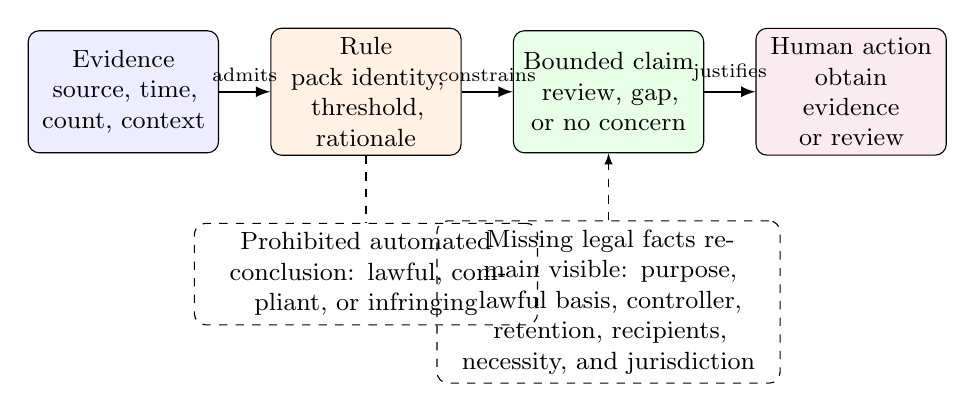
\begin{tikzpicture}[
  node distance=0.65cm,
  box/.style={draw, rounded corners, align=center, text width=0.18\textwidth, minimum height=1.55cm, font=\small},
  note/.style={draw, dashed, rounded corners, align=center, text width=0.34\textwidth, font=\small},
  arrow/.style={-latex, thick}
]
\node[box, fill=blue!7] (evidence) {Evidence\\source, time, count, context};
\node[box, fill=orange!10, right=of evidence] (rule) {Rule\\pack identity, threshold, rationale};
\node[box, fill=green!9, right=of rule] (claim) {Bounded claim\\review, gap, or no concern};
\node[box, fill=purple!8, right=of claim] (action) {Human action\\obtain evidence or review};
\draw[arrow] (evidence) -- node[above,font=\scriptsize]{admits} (rule);
\draw[arrow] (rule) -- node[above,font=\scriptsize]{constrains} (claim);
\draw[arrow] (claim) -- node[above,font=\scriptsize]{justifies} (action);
\node[note, below=0.85cm of claim] (missing) {Missing legal facts remain visible: purpose, lawful basis, controller, retention, recipients, necessity, and jurisdiction};
\draw[dashed,-latex] (missing) -- (claim);
\node[note, below=0.85cm of rule] (prohibited) {Prohibited automated conclusion: lawful, compliant, or infringing};
\draw[dashed] (rule) -- (prohibited);
\end{tikzpicture}
\caption{Evidence-to-action conceptual boundary}
\label{fig:conceptual-boundary}
\end{figure}

The model is directional. Evidence constrains which rule can run; the rule constrains the claim; and the claim constrains the action that can be justified. The interface must not reverse this logic by beginning with a desired compliance label and searching for a supporting count. Nor should it allow an action such as reporting an application to imply that the underlying legal question has already been resolved.

Uncertainty enters at each transition. Evidence may be incomplete, a rule may be a research baseline, a claim may omit legally decisive context, and an action may require professional judgement. Rather than compressing these uncertainties into one confidence score, Privacy Lens retains categorical source, explicit missing fields, rule metadata, and textual boundaries. This choice follows the reviewed literature's emphasis on contextual interpretation and calibrated reliance while remaining implementable in a deterministic prototype.

The model also explains the division of evaluation. Admission and replay tests concern evidence. Threshold and pack fixtures concern rules. Projection and screenshot checks concern claims. Participant and professional-review studies would concern actions and reliance. Keeping these layers separate allows the thesis to answer its engineering questions without presenting unevaluated human or legal outcomes as completed results.

\subsection{Store Delivery as a Trust Boundary}

Application-store readiness includes more than a successful APK. Google Play uses Android App Bundles for new application delivery, requires current target API levels, and requires developers to complete a Data safety declaration \cite{androidbundle2026,playtarget2026,playdatasafety2026}. Signing identity, a public privacy-policy URL, support contact, screenshots, listing text, and console review remain owner-controlled steps. A research build can be an initial submission candidate while still being unpublishable until these external obligations are completed.

\subsection{Synthesis}

The literature yields a precise design requirement: a privacy-review system must preserve the boundary between an observation and the authority of the claim made from it. Android research defines the acquisition constraint; regulatory sources define the missing legal context; HCI and accessibility sources define the communication constraint; and rule-system research defines the maintenance constraint. The following chapter converts this model into explicit requirements, design alternatives, and evidence contracts.

\input{Iteration-V2/Chapter3/chapter-03-15}
\input{Iteration-V2/Chapter4/chapter-04-15}
\input{Iteration-V2/Chapter5/chapter-05-15}
\input{Iteration-V2/Chapter6/chapter-06-15}
\input{Iteration-V2/Chapter7/chapter-07-15}
{\small
\bibliographystyle{ieeetr}
\bibliography{reference}
}
\end{document}
